\documentclass[oneside, 10pt, a4paper, twocolumn]{article}

\usepackage[small]{titlesec}
\usepackage{fancyhdr}
\usepackage{textcomp} 
\usepackage{amssymb}
\usepackage{amsmath}
\usepackage{amsthm}
\usepackage{amscd}
\usepackage{amsfonts}
\usepackage{mathrsfs}
\usepackage{graphicx}
\usepackage[utf8]{inputenc}
\usepackage[T1]{fontenc}
\usepackage[english]{babel}
\usepackage{color}
\usepackage{braket}
\usepackage{caption}
\usepackage{minitoc}
\usepackage{lmodern}
\usepackage{microtype}
\usepackage{booktabs}
\usepackage{epsf}
\usepackage{epstopdf}
\usepackage{bm}
\usepackage{pdflscape}
\usepackage{varioref}
\usepackage[square,sort]{natbib}
\usepackage{authblk}
\usepackage[columnwise, switch]{lineno}
\usepackage{authblk}
\usepackage{mwe}    % loads »blindtext« and »graphicx«
\usepackage{subfigure}
\usepackage{multirow} % Allows to write multiple rows
\usepackage{floatrow}
\usepackage{graphicx,mathtools,kantlipsum}
\usepackage[utf8]{inputenc}
\usepackage{hyperref}
\usepackage{pdfpages}
\newcommand{\jmg}[1]{{\color{red}  \textbf{[Jorge: #1]}}}


\hypersetup{
     colorlinks   = true,    
     citecolor     = blue    % hypersetup for references
}

\DeclareGraphicsExtensions{.jpg, .pdf, .png}

\newcommand{\beginsupplement}{%
        \setcounter{table}{0}
        \renewcommand{\thetable}{S\arabic{table}}%
        \setcounter{figure}{0}
        \renewcommand{\thefigure}{S\arabic{figure}}%
     }

%=================================================================
%%=================================================================
\begin{document}


% Max ~2500 words for 'Report' and ~1500 words for 'Brief report' in main text

\title{Causal dynamical modelling predicts \\ novel regulatory genes \\ of FOXP3 in human regulatory T cells}
\date{}
\author{Rucha Sawlekar\thanks{These authors contributed equally to this work.} \thanks{Luxembourg Centre for Systems Biomedicine, University of Luxembourg, 6 Avenue Du Swing, L-4367 Belvaux, Luxembourg.} , Stefano Magni$^{*\dagger}$, Christophe Capelle$^{*}$\thanks{Luxembourg Institute of Health, 29 Rue Henri Koch, L-4354 Esch- Sur-Alzette, Luxembourg.} , Alexandre Baron$ ^{\ddagger} $, Ni Zeng$ ^{\ddagger} $, Laurent Mombaerts$ ^{\dagger} $,  Zuogong Yue\thanks{University of New South Wales, Kensington NSW 2052, Australia.} , Ye Yuan\thanks{School of Artificial Intelligence and Automation, Huazhong University of Science and Technology, Wuhan 430074, China.} , Feng Q. He\thanks{Co-corresponding authors of this work. Emails: feng.he@lih.lu, jorge.goncalves@uni.lu.} $ ^{\ddagger} $, and Jorge Gon\c{c}alves$ ^{\|\dagger}$\thanks{Department of Plant Sciences, University of Cambridge, Downing Street, Cambridge CB2 3EA, United Kingdom.}
% <-this % stops a space
% <-this % stops a space
%\thanks{Manuscript received April 19, 2005; revised September 17, 2014.}
}
\maketitle

\newpage

\hypersetup{
      linkcolor = blue % hypersetup for section references
}

%=================================================================
%%=================================================================

\abstract   % MAX 150 words
Regulatory T cells (Tregs), characterized as a CD4+CD25+FOXP3+ subset of T cells, are vital to the induction of immune tolerance and the maintenance of immune homeostasis. While target genes of Treg master regulator FOXP3 have been identified, the upstream regulatory machinery of FOXP3 still remains largely unknown. Here we dynamically model {\em causal} relationships among genes from available time-series genome-scale datasets, to predict direct or indirect regulatory genes of FOXP3 in human primary Tregs. From the whole genome, we selected five top ranked candidates for further experimental validation. Following knockdown, three out of the five candidates indeed showed significant effects on the mRNA expression of FOXP3. Further experiments showed that one out of these three predicted candidates, namely nuclear receptor binding factor 2 (NRBF2), also affected FOXP3 protein expression. These results 
%study 
open new doors to identify potential new mechanisms of immune related diseases.
% novel potential upstream regulatory candidates for  genes of interests.


\vspace{0.5cm}

% MAXIMUM = 10 for "cell systems" journal
\textbf{Keywords:} regulatory T cells, FOXP3, dynamical modelling, humans, time-series analysis, network inference, regulatory network,  transcriptomic data, system identification, causal network.

\vspace{0.5cm}

%=================================================================
Regulatory T cells (Tregs) are a key player of the immune system, which in turn plays a crucial role in a wide range of diseases. The transcription factor FOXP3 is the master regulator of Tregs and thus we focus on it. Genes regulating FOXP3 are still largely unknown and identifying them may be vital for developing new immunotherapeutics. In this work we aim at computationally screening the genome for such potential regulatory genes, and then at experimentally proof-of-concept testing some of the predictions obtained.

Tregs perform immunosuppression of self-reactive lymphocytes to induce immunological self-tolerance and maintain homeostasis \citep{janeway2012immunobiology, Li2015,Josefowicz2012}. Tregs are involved in different types of diseases, such as autoimmune diseases \citep{Dejaco2006, Fehervari2004, Sakaguchi2006}, cancer \citep{Shang2015, Tanaka2017,franchina2018survival}, infectious diseases \citep{Joosten2008, StephenVictor2017}, neurodegenerative diseases \citep{Baruch2015, He2013} and others \citep{Cools2007}. 

The transcription factor FOXP3  has been shown to play a decisive role for the development and function of Tregs \citep{Ziegler2006}. This gene is expressed specifically in CD4$^{+}$CD25$^{+}$ Tregs \citep{hori2003control, rudensky2011regulatory}. Altered expression of FOXP3 has been found in various types of autoimmune diseases \citep{liu2013ipex} and tumors \citep{cunha2012foxp3, martin2010human,szylberg2016role}. 
Genetic mutations in FOXP3 result in autoimmunity and inflammatory syndromes, both in humans and in mice \citep{mayer2014few, mercer2009biology,Fontenot2003,Khattri2003}. Most of the experimental evidence indicates that FOXP3 deficiency is responsible for IPEX (immunodysregulation polyendocrinopathy enteropathy X-linked) syndrome which is a rare disease caused by dysfunction of Tregs \citep{bennett2001immune}.

Target genes of FOXP3 have been 
%intensely studied and identified
identified through intensive studies~\citep{Marson2007, Zheng2007, ZhengRudensky2007}. Meanwhile, progress in high-throughput technical developments, such as ChIP-seq and ChIP-Chip, have started to illuminate 
% shed some light on 
genetic and epigenetic mechanisms regulating expression or protein stability of FOXP3 \citep{Floess2007, Fu2012, Miyara2007, Schmidt2012, CHEN2013272,GaoE3246}. Interestingly, the majority of known upstream regulators of the expression of FOXP3 are general regulatory genes, e.g., those controlling interleukin signaling pathways (IL2, IL4, IL6 and so on) and cell surface receptors (TGFB)  \citep{Lal2009}. Those 
% general regulatory 
genes tend to regulate a large number of genes far beyond FOXP3, which might cause significant unwanted side effects when being targeted. 

More specific upstream genes regulating FOXP3 are still largely unknown. Identifying these regulators of FOXP3 may be crucial for developing new immunotherapeutics against autoimmune and other related diseases. Unbiased experimental screening of the whole genome for such upstream regulators is almost impossible with current experimental approaches. However, such tasks can be efficiently performed computationally. This is the goal of this work.

The models trained in this work are based on microarray data of the whole-genome mRNA expression in isolated human Tregs~\citep{he2012plau}. Tregs from two different donors were stimulated at time zero with anti-CD3/-CD28/IL2, and measurements were taken at time zero followed by sampling every twenty minutes over a period of six hours (19 time points in total). After the pre-processing of the data, as outlined in column 1 of Fig.~\ref{fig:ComputationalFigure}a and described in Supplementary Section~\ref{SISubSection:NormAndFiltering}, there were 
%approximately 15,000 
13601 transcripts/probe sets left, corresponding to 7826 genes. A gene can correspond to multiple transcripts, each measured by a separate probe set; from now on for simplicity we will only use the term transcripts and omit the term probe sets. The role of the computational modelling was to reduce this number to 5 genes, reflecting our available experimental resources for validation.

%\begin{figure*}
%  \mbox{   \centering
%    %----------------  FIGURE : Project work-flow   ----------------
%    \subfigure[Overview of the different stages of the computational approach, %from raw time-series transcriptomic data to the resulting ranking of genes 
%    % probe sets 
%    likely to regulate FOXP3. The abbreviation ACT stands for activator, REP for repressor. \label{fig:workflow}]{\includegraphics[scale=0.53]{Fig1a_ProjectWorkflow_130120.pdf}}  
%    \quad
%}
%    %----------------  FIGURE : Fit. score Vs gene number   ----------------
%     \mbox{
%     \centering
%    \subfigure[Fitness score versus gene number for all genes. Two regimes are visible: a group of genes showing a steep decrease in fitness, and a much larger group showing an almost linear decrease in fitness. The panel on the top right corner shows a magnification of the region with the top ranked genes. The rank of the first 176 genes is reported as Supplementary Table 1.     \label{fig:fitnessScoreVsGeneNumber}]
%    {\includegraphics[scale=0.30]{FitScoreVSGeneNumber_Treg2_7020genes_4.pdf}}  
%    \quad  \hspace{20pt}
    %----------------  FIGURE : Regulators of FOXP3   ----------------
%    \subfigure[Overview of predicted regulators of FOXP3, which were tested \textit{in vitro}.
%     \label{fig:regulatorsOfFOXP3}]
%    {\includegraphics[scale=0.36]{Fig1c_Regulators_of_FOXP3}}
%  }
%  \caption{\textbf{Overview of the computational data analysis resulting in hypothesized regulators of FOXP3 for subsequent \textit{in vitro} testing.}  
%  }
%  \label{fig:ComputationalFigure}
%\end{figure*}

\begin{figure*}
    \centering
    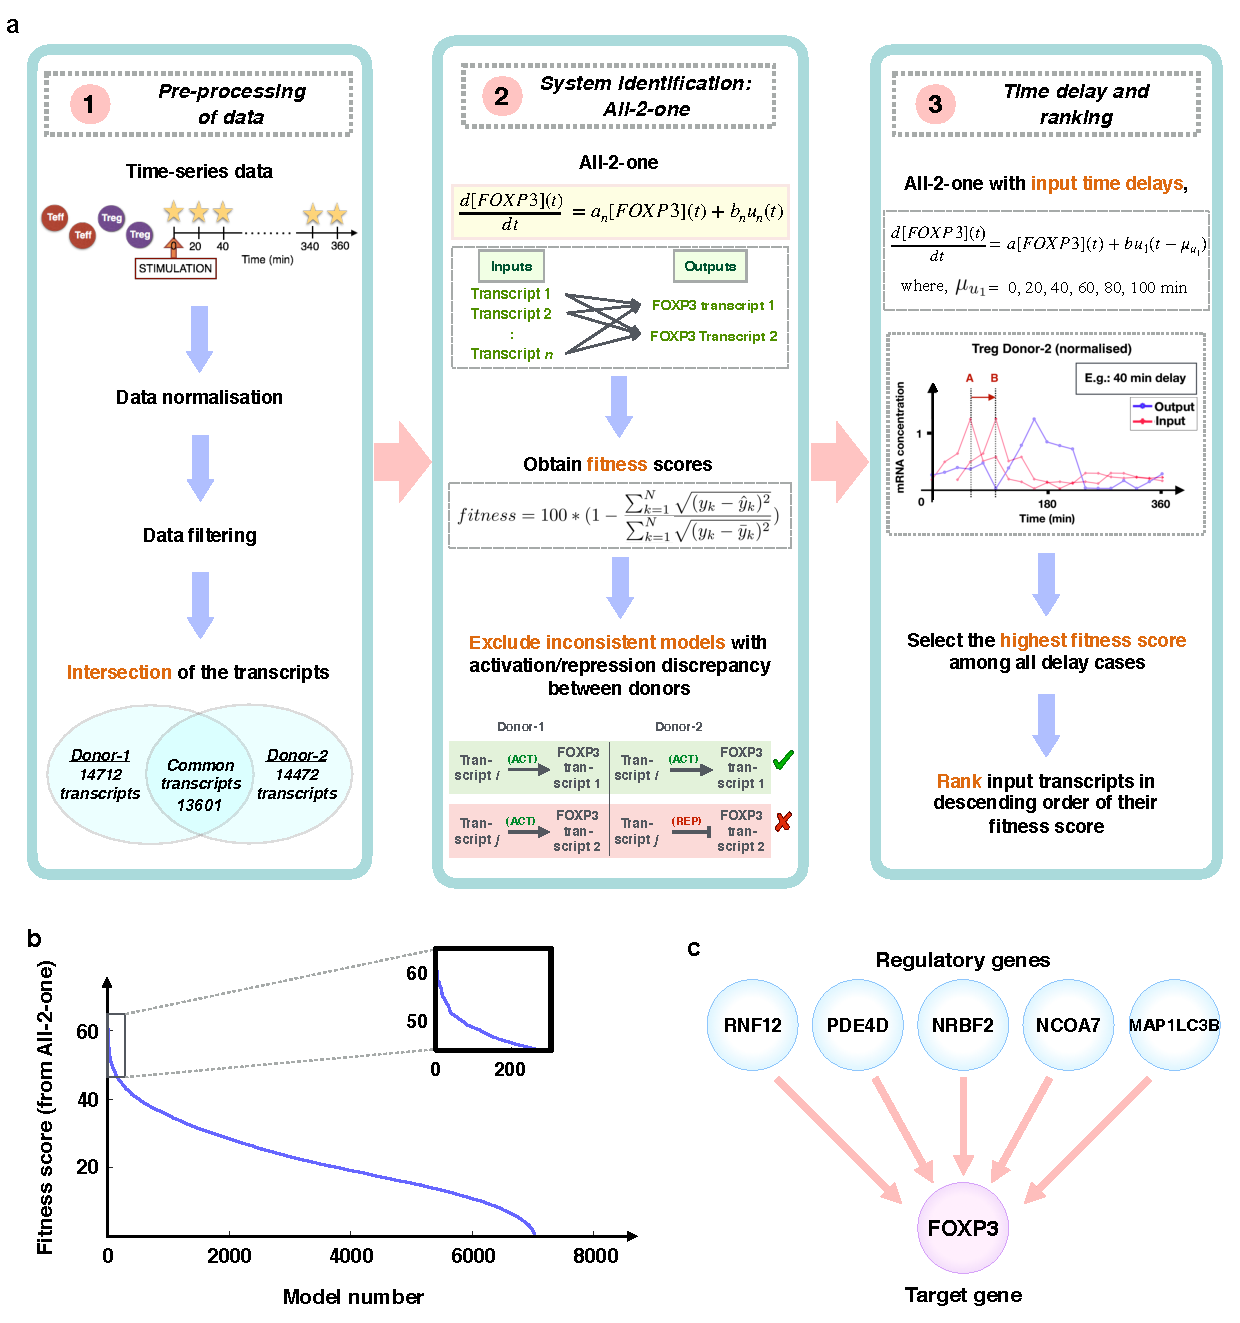
\includegraphics[scale=0.73]{Fig1_AllInOne.pdf}
  \caption{\textbf{Causal dynamical modelling pipeline resulting in hypothesized regulators of FOXP3 for subsequent \textit{in vitro} testing.} \textbf{(a)} Overview of the different stages of the computational approach, from raw time-series transcriptomic data to the resulting ranking of genes likely to regulate FOXP3. The abbreviation ACT stands for activator, REP for repressor. \textbf{(b)} Fitness score versus model number for each transcript paired with each of the two available FOXP3 transcripts. Two regimes are visible: a group of models showing a steep decrease in fitness, and a much larger group showing an almost linear decrease in fitness. The box on the top right corner of this panel shows a magnification of the region with the top ranked models. The ranking of models directly translate in ranking the input transcripts. The rank of the first 176 transcripts is reported as Tab.~\ref{SupTabComputational}. \textbf{(c)} Overview of predicted regulators of FOXP3 which were tested \textit{in vitro}.
  }
  \label{fig:ComputationalFigure}
\end{figure*}

Existing models capture known regulations 
% Existing models in the literature mainly capture already known regulations 
of genes by FOXP3 \citep{VanDenHam2008, Hong2011, Carbo2013, Carbo2015}, so they were not useful in finding novel regulators of FOXP3. Hence, we need to fit new models from data that capture {\em causality}, i.e., that identifies those genes that {\em cause} changes in FOXP3. Here, we take advantage of a relatively large number of available time-series Treg samples to fit dynamical models. In particular, ordinary differential equations are mathematical abstractions that capture both dynamics and causality, and help build testable hypotheses in experiments. Our models take time-series expression values of the whole genome as inputs and FOXP3 as the single output (target). 

There is always a trade-off on the choice of model complexity. With rich data, models can be complex, providing detailed information of mechanisms of action. However, with limited data, complex models can easily overfit and introduce bias, resulting in large numbers of false negatives. In our case, with only a single time-series experiment and limited resources for validation, we consider the simplest dynamical model: first-order linear time-invariant (LTI) systems, a well established modelling strategy~\citep{Mombaerts2019, Muller2019,Dalchau2012, Herrero2012, Mombaerts2016}.
Moreover, to scale the method to the whole genome, we built a large number of simple  pairwise models (one per gene), testing whether each gene on its own could regulate FOXP3. A model associated with a particular $gene$ is given by
$$\frac{d \mbox{FOXP3}(t)}{dt} = a \cdot \mbox{FOXP3}(t) + b\cdot gene(t)$$
The left-hand side of the equation is the derivative of FOXP3 expression over time, i.e., the rate of change of the concentration of FOXP3. Finally, we searched for parameters $a,b$ that best fitted the data. This procedure was repeated for all 
%\textasciitilde 15000 
13601 transcripts. Given the simplicity of the models, high fit means high confidence that such regulation of FOXP3 may indeed exist. 
This method was summarised in column 2 of Fig.~\ref{fig:ComputationalFigure}a and further details were in Supplementary Sections~\ref{SISubSection:One-2-one} and~\ref{SISubSection:All-2-one}.

Potential regulators of FOXP3 identified here may or may not be transcription factors. Indeed, our models can capture both direct or indirect regulations of FOXP3. 
Indirect regulations involve other molecules and typically require larger dimensional models to capture the dynamics of intermediate steps. To avoid increasing model complexity and still consider indirect regulations, we introduced a single time delay $\tau$ in the input signal
$$\frac{d \mbox{FOXP3}(t)}{dt} = a \cdot \mbox{FOXP3}(t) + b\cdot transcript(t-\tau)$$
Hence, each model had a total of three parameters. Finally, transcripts 
% probe sets 
were ranked according to how likely they are to regulate FOXP3. This was illustrated in column 3 of Fig.~\ref{fig:ComputationalFigure}a and described in Supplementary Section~\ref{SISubSection:All-2-one}. 

%To be consistent, our method should rank in high positions at least some genes already known to be involved in pathways regulating FOXP3. To verify that this is the case, we performed Gene Set Enrichment Analysis (GSEA) \citep{Subramanian2005, Mootha2003} on the full list of 7030 genes ranked by our algorithm. 
%Because we had a ranked genes list, we run a “GSEAPreranked” analysis, with default parameters. 
%The GSEA method considers known sets of genes from the literature, and for each set it verifies if the preranked list of genes provided by the user shows any enrichment of gene names in the top (or bottom) of the list. We included from the standard database employed by GSEA (Molecular Signatures Database, MSigDB) a total of 8054 sets of genes. As a result, we obtained that among these sets, only 3 gene sets were significantly enriched in the top of our list with false discovery rate < 5 $\%$. These 3 corresponded to the following sets: genes up-regulated in comparison of 1) untreated CD4 T cells at 0 h versus the cells treated with IL4 and anti-IL12 at 4 h, 2) same but at 2h, 3) same but versus the untreated cells at 2 h. All these three sets of genes are from \cite{Elo2010}, which studies in detail the transcription kinetics initiated by cytokine IL-4 in early differentiation of Th2 cells. We thus conclude that the ranking of genes produced by our method is relevant w.r.t. the biological system under investigation. For an extended discussion of our GSEA analysis, see Supplementary Section \ref{SISubSection:GSEA}.

We decided to focus on the top 176 transcripts (Tab.~\ref{SupTabComputational}) 
% probe sets 
out of 7030. 
Fig.~\ref{fig:ComputationalFigure}b showed a significant change in the rate of change of the fitness values, i.e., a kink, after the first 176 transcripts. 
% probe sets. 
Of those, there were 161 distinct genes, since 15 of the 176 transcripts 
% probe sets 
corresponded to the same genes. These genes covered fitness values ranging from 62 to 46 (the higher of the fitness value, the better; 100 is perfect fit). 
Among the remaining 161 top ranked genes, FOXP3 is known to bind the promoters of 59 genes \citep{Sadlon2010}, and 38 genes are reported to be differentially expressed in human Tregs compared to CD4$^{+}$CD25$^{-}$ effector T cells (Teffs)~\citep{Sadlon2010}. For 15 genes, both statements were true. 
% the proteins of 15 out of the 161 top ranked genes have been shown to bind to FOXP3 and their mRNA are differentially regulated, compared to CD4$^{+}$CD25$^{-}$  effector T cells (Teffs)~\citep{Sadlon2010}. 
As a first literature validation test, this shows that the predicted top ranked genes are indeed involved in the regulatory pathways related to FOXP3, already supporting the relevance of our prediction.

%To be consistent, our method should rank in high positions at least some genes already known to be involved in the FOXP3-related pathways. To verify that this is the case, we compared our top ranked genes with a study which looks at genome-wide targets of FOXP3 in human Tregs \citep{Sadlon2010}. From the 176 genes in our list, there were 15 genes that were in the list more than once (different probe sets). From the remaining 161, there were 59 genes that were also \citep{Sadlon2010} identified as genes that can be bound by FOXP3, and 38 that were differentially regulated, compared to CD4$^{+}$CD25$^{-}$  effector T cells (Teffs). For 15 genes from our list both were true. This comparison supports the fact that our prediction is identifying, as top ranked genes, genes that are indeed involved in the regulatory pathways which are related to FOXP3, thus providing support for the reliability of our prediction. We thus conclude that the ranking of genes produced by our method is relevant w.r.t. the biological system under investigation.

Next, we experimentally validated some of the 161 top ranked genes in primary human Tregs (Fig.~\ref{fig:ExperimentalFindings}a). Considering the available resources, we selected only 5 genes: \textit{NCOA7}, \textit{MAP1LC3B}, \textit{NRBF2}, \textit{PDE4D} and \textit{RNF12} (Fig.~\ref{fig:ComputationalFigure}c). The choice of these 5 genes was mostly based on a smooth dynamical profile with rise and fall dynamics ahead of FOXP3, and a diversity of activity in different cell parts. 

%Obviously \citep{d2000genetic}, the subsequent step was to test some of these hypotheses experimentally. 

Our experimental results showed a  successful knockdown of \textit{MAP1LC3B}, \textit{NCOA7} and \textit{NRBF2} using siRNA specifically targeted against the corresponding gene relative to a control scrambled siRNA in primary human Tregs (Fig.~\ref{fig:ExperimentalFindings}b, c and d). Excitingly, knockdown of \textit{MAP1LC3B}, \textit{NCOA7} and \textit{NRBF2} down-regulated the transcript expression of \textit{FOXP3} in Tregs (Fig.~\ref{fig:ExperimentalFindings}b, c and d). The dynamics of \textit{FOXP3} expression following siRNA treatment was slightly different for the three candidates. 
% Note that the timing when the effect on \textit{FOXP3} expression was visible, was slightly different for the three candidates. 
For the other two candidates, \textit{PDE4D} and \textit{RNF12}, although we successfully knocked down their mRNA expression, there was no clear effect on the mRNA expression of FOXP3 (data not shown here). 


\begin{figure*}
\centering
  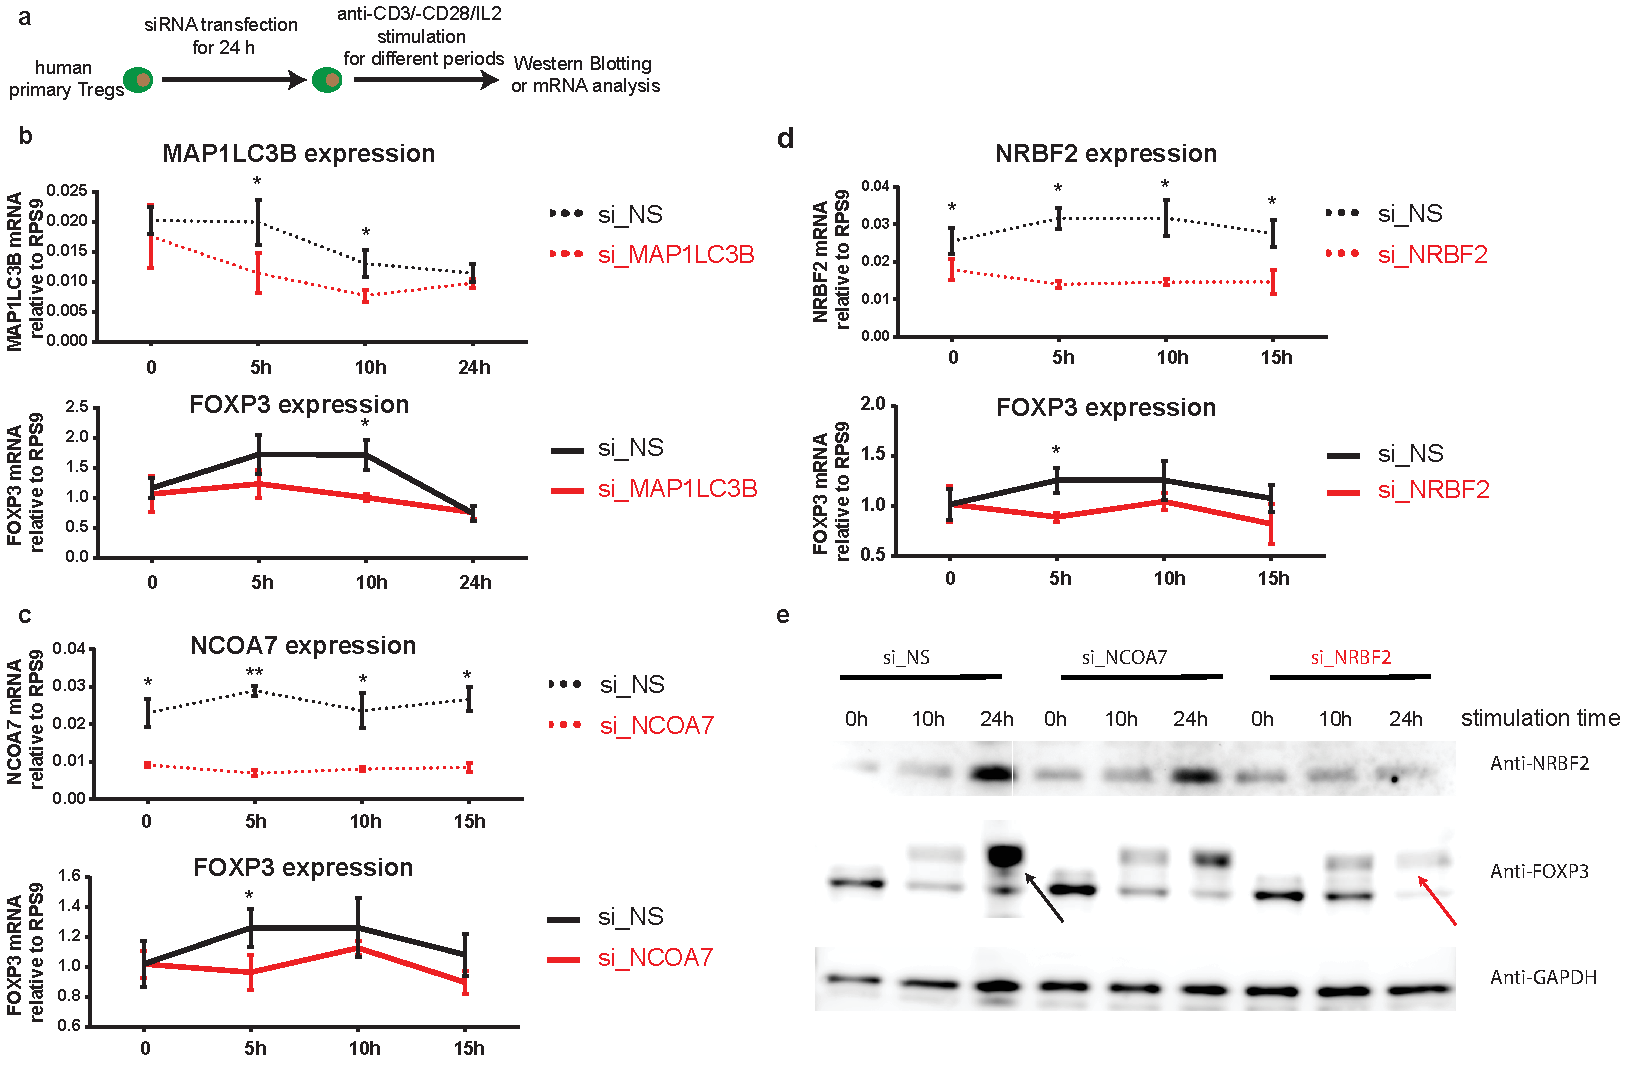
\includegraphics[scale=0.57]{Fig2_Exp.pdf}
  \caption{\textbf{Experimental validation of predicted candidates.} 
\textbf{(a)} Experimental scheme of the knockdown experiments. The predicted candidate genes were knocked-down by siRNA transfection in primary human Treg for 24h, followed by CD3/CD28/human rIL-2 stimulation. 
\textbf{(b)} Quantitative real-time PCR results for the knockdown of MAP1LC3B in human primary Treg and the corresponding FOXP3 expression. Control scrambled non-specific knockdown (si$\_$NS) is shown in black and the specific knockdown (si$\_$MAP1LC3B) in red. Statistical significance was determined using Student t-test, *p<0.05, **p<0.01, and ***p<0.001.
\textbf{(c)} Quantitative real-time PCR results for the knockdown of NCOA7 in human primary Tregs and the corresponding FOXP3 expression. Control knockdown (si$\_$NS) is shown in black and the specific knockdown (si$\_$NCOA7) in red.
\textbf{(d)} Quantitative real-time PCR results for the knockdown of NRBF2 in human primary Tregs and the corresponding FOXP3 expression. Control knockdown (si$\_$NS) is shown in black and the specific knockdown (si$\_$NRBF2) in red.
\textbf{(e)} Western Blot showing the protein expression of NRBF2 and FOXP3 in human primary Tregs transfected with si$\_$NCOA7, si$\_$NRBF2 or control siRNA (si$\_$NS). The bands of interest are highlighted by black (si$\_$NS) or red arrows (si$\_${NRBF2}).
}  \label{fig:ExperimentalFindings}	
\end{figure*}


Next, we tested the potential effect on protein production. All our predictions were based on models built from mRNA data, not protein expression. Due to the limited availability of reliable antibodies on MAP1LC3B, we performed Western Blotting analysis to test the effects of knockdown of only NCOA7 and NRBF2 on the protein expression of FOXP3. So far, we could only successfully demonstrate the downregulation of NRBF2 protein expression. Notably, in line with the mRNA results, dowregulation of NRBF2 protein expression indeed reduced the expression of certain isoforms of the FOXP3 protein (Fig.~\ref{fig:ExperimentalFindings}e), possibly due to altered alternative splicing  \citep{Allan2005}. All these experiments have been successfully repeated in Tregs isolated from peripheral blood of 6 to 8 healthy donors, depending at which level (protein or mRNA or both) the validation was performed. The effect was not observed in 1 or 2 of the tested donors possibly due to the heterogeneous nature of human individual samples.

NRBF2 is known to regulate the activity of VPS34 \citep{Lu2014}. Moreover, T-cell specific depletion of VPS34, significantly impaired the maintenance and the suppressor function of Tregs \citep{Parekh2013}. Our results, together with these published works, already indicate that NRBF2 might be a promising upstream regulator that modulates the expression of FOXP3.

One limitation of our computational approach is that, being based on a linear dynamics, it might miss complex non-linear interactions. Furthermore, since our method checks one transcript at a time as a potential regulator of FOXP3, it might miss interactions requiring cooperativity among several regulators at a time. Due to limited amount of data available, however, higher model complexity is likely to lead to overfitting and false positives. Since the ground truth behind the biological system that generated this data is unknown, the safest route is to consider low complexity models, as we did here. 
% We addressed these limitations more widely in Supplementary Section~\ref{SI:ComputationalMethods}. 
Moreover, many transcription factors are regulated at the post-transcriptional level, which are not captured by our models and predictions (since the models are built on transcriptional data alone). 

In summary, we applied dynamic modelling techniques to predict upstream regulatory genes of FOXP3, the master regulator of Tregs. Then, we experimentally validated the predicted effect of a handful of genes. All three genes \textit{MAP1LC3B}, \textit{NCOA7} and \textit{NRBF2} down-regulated the transcript expression of \textit{FOXP3}. Moreover, dowregulation of NRBF2 protein expression reduced the expression of FOXP3 protein. 
Although NRBF2 knockout mice do not show spontaneous autoimmune phenotypes, NRBF2 positively regulates the autophagy process \citep{Lu2014}, which has been widely associated with  autoimmune diseases \citep{GIANCHECCHI2014}. Moreover, an integrative meta-analysis from around 72 million functional associations shows that NRBF2 is ranked as the sixth candidate gene related to juvenile rheumatoid arthritis \citep{Rouillard2016}, one of the classic autoimmune diseases. Overall, our results enhance our understanding of the upstream regulatory mechanisms of FOXP3, with the potential to develop new immunotherapeutics. Our results are solely derived from {\em human} primary T cells and therefore guarantee their application potential in medicine.

Potential future developments 
%on the experimental side 
include, but are not limited to, the following: (1) to experimentally test  \textit{MAP1LC3B}, \textit{NCOA7} and \textit{NRBF2} \textit{in vivo} in animal models, for example using corresponding whole-body or T-cell-specific knockout mice under homeostatic and pathological conditions; (2) to experimentally investigate additional regulators of FOXP3 from the predicted list of top ranked genes; (3) to apply the same computational approach to identify regulators of another important gene of relevance for Tregs, e.g., CTLA4; (4) if additional suitable time-series data with even shorter sampling intervals for this system would be available in the future, we would apply more complex modelling paradigms than the one employed in this work, with the aim of identifying more complex gene regulatory interactions possibly with even higher predictive power; (5) finally, we could consider to extend in the future our computational approach to infer gene regulations from single-cell RNA-seq data, as pioneered by other works such as \citep{Chan2017} and \citep{Ocone2015}.


%=================================================================


\section*{Acknowledgements}    
\label{Section:Acknowledgements}
This work was supported by the Luxembourg National Research Fund (FNR) CORE grant, ref  CORE/14/BM/8231540/GeDES. 
Stefano Magni and Christophe Capelle are supported in part by the FNR PRIDE DTU CriTiCS, ref 10907093. 
Jorge Gon\c{c}alves is partly supported by the 111 Project on Computational Intelligence and Intelligent Control, ref B18024. 
Feng He is partly supported by the Luxembourg Personalized Medicine Consortium (PMC), FNR individual AFR or AFR-RIKEN bilateral program ref 9989160 and TregBAR, \mbox{PRIDE DTU NextImmune ref 11012546.}

%=================================================================

% unsrtnat
% agsm
\bibliographystyle{apalike}
\bibliography{TregBibliography}

\clearpage

\newpage
\section*{SUPPLEMENTARY MATERIAL}
%\\ $ \bigstar  $ STAR METHODS}


%======================================
\section{COMPUTATIONAL METHODS DETAILS}   
\label{SI:ComputationalMethods}
%======================================


\subsection{Time-Series Data Normalisation and Filtering}    
\label{SISubSection:NormAndFiltering}

As shown in Fig.~\ref{fig:ComputationalFigure}, first of all we obtained the raw data corresponding to Tregs cells from the online supplementary material of \citep{he2012plau}. Therein, microarray measurements were performed for every 20 min over the period of 6 h, after stimulation by anti-CD3/CD28/human rIL2 at time 0 h on Treg cells from two donors (here referred to as donor-1, donor-2). This data contained 54,676 transcripts/probe sets for each donor, mapping various transcript variants of almost each gene in the whole genome. For simplicity, in the text we only use the term transcript and skip the more technical term probe set, keeping in mind that they are in a one-to-one relation, thus exchangable.

Before applying any system identification technique, these time-series data need to be pre-processed. This involves normalising the data using the gcrma algorithm \citep{wu2010description} which is implemented in MatLab. For this and all the other computational work of this work, MatLab versionS R2016a, R2016b and R2017a were used. The normalised data were then subject to filtering. Firstly, we applied affymetrix flag filter, where any probe set was removed if marked as \textit{absent} in every measurement taken at each instant of time. Conversely, we kept all the probe sets for which at least one measurement taken at any instant of time was marked with \textit{marginally present} or \textit{present}. The second filter applied removed the probe sets for which the average intensity (of the mRNA expression, which depends on the normalisation used above) is $ < $50, or the largest intensity among measurements performed at any time is $ < $100 (in the arbitrary units used by the gcrma algorithm). After this filtering, 14712 probe sets were left for donor-1 and 14472 probe sets for donor-2. The intersection of these two ensembles led to a common set of 13601 probe sets left.


\subsection{One-2-one Method}
\label{SISubSection:One-2-one}

{Here, we used the methodology presented in \citep{Mombaerts2019} to identify candidates regulators for FOXP3. This modeling strategy uses Linear Time-Invariant (LTI) models to capture the dynamics describing the rate of change of the selected transcript with respect to another input transcript. A linear modelling paradigm offers advantages when data are scarce. In particular, although linear models do not provide detailed functioning of the whole network, they are capable of identifying regulatory interactions with a reliable degree of precision (see below). A LTI model can be generally represented by the following set of equations:
\begin{equation}
\begin{array}{l}
\frac{dx}{dt}(t) = A x(t) + B u(t) \\
    y(t) = Cx(t) \, .
\end{array}
\label{SI:Eq:LTImodel}
\end{equation}\\
The model investigates whether the rate of change of the gene expression of a particular transcript $y(t)$ depends on the gene expression of another transcript $u(t)$. In particular, $u(t)$ and $y(t)$ represented the time series of the gene expression over time of a potential regulator of FOXP3 and FOXP3, respectively. The variable $x(t)$ represented internal dynamics (translation, transcription, etc...) that interacted with the modelled output and were required for the behaviors observed, but were not explicitly included in the model. The dimension of the vector $x(t)$ defines the model order: in general it can be a 1-dimensional vector (direct regulation or relatively slow dynamics compared to internal dynamics), or a multi-dimensional vector (the regulation happens through intermediate steps that introduce delays and cannot be ignored). 
% This was repeated for all potential candidates to identify potential regulators of FOXP3. 
\\ \\
Estimating a model involves finding $A$, $B$ and $C$ which produce a vector $y(t)$ as close as possible to the real expression data. On one hand, complex nonlinear models have the potential to capture the dynamical relationships between genes with great precision. On the other hand, high complexity can lead to overfitting (fitting noise instead of dynamics) without sufficient data or detailed knowledge such as the network topology or types of nonlinear interactions. Here, we restricted the model order to one as it was optimally estimated in \citep{Mombaerts2019}. Hence, $A$, $B$ and $C$ were scalars. Furthermore, since $y$ is the measurement of a single state, $C$ then consists of a scalar of value 1. System identification was performed using the function 'pem' implemented in MATLAB to minimise the prediction \mbox{error \citep{Ljung1998}.} \\ \\
Each model was characterized by a performance index that represents the capability of the model to describe the input-output relationship. To do so, we used the fitness:
\begin{equation}
fitness = 100 * \left(1 - \frac{\sum_{k=1}^{N} \sqrt{(y_k - \hat{y}_k)^2}}{\sum_{k=1}^{N} \sqrt{(y_k - \bar{y}_k)^2}}\right) \\
\label{fitness}
\end{equation}\\
where $y_k$ represented the simulated data (output), $\bar{y}$ the average value of the simulated data, and $\hat{y_k}$ the estimated output. MATLAB function $compare$ can be used to compute the fitness of the model. A fitness equal to 100\% corresponds to a perfect identification. A high fitness suggests that most of the dynamics was captured. \\ \\
Then, to investigate the potential regulators of FOXP3, a collection of 1st order LTI models was estimated from each of the transcripts to FOXP3. In each case, the parameters were estimated so that they together provided the best possible fit to FOXP3 time course data. This step took the following form:\\
\begin{equation}
\begin{array}{l}
\frac{d[FOXP3](t)}{dt} = a_1 [FOXP3](t) + b_1 u_1(t) \\ \\
\frac{d[FOXP3](t)}{dt} = a_2 [FOXP3](t) + b_2 u_2(t) \\ \\
... \\ \\
\frac{d[FOXP3](t)}{dt} = a_n [FOXP3](t) + b_n u_n(t) \\ \\
\end{array}
\label{All-2-oneEq}
\end{equation}\\
where $n$ corresponds to the amount of candidates. Each model was characterized by a fitness metric that ranges from 0 to 100\%, representing its capability of describing the original regulatory system between genes. A gene, therefore, would be further considered as a regulator for FOXP3 if the model obtained using one of its transcripts was capable of reproducing the expression profile of FOXP3 with a sufficient degree of precision, which should be characterized by a high goodness of fit, as defined above. \\ \\
Additionally, we derived the mathematical expression of the dynamics of FOXP3 to explicitly include a delay in the modelling, such that it took the following form:\\
\begin{equation}
\frac{d[FOXP3](t)}{dt} = a [FOXP3](t) + b u_1(t-\mu_{u_1}) \\ \\
\label{DelayEq}
\end{equation}\\
where $\mu_{u_1}$ is a delay chosen between $0$ min and $100$ min, with steps of $20$ minutes. The choice $\mu_{u_1} = 0$ min reduces the models to the particular case employed above.


%\subsection*{Evaluation of Performances of the One-2-one method}
%\label{SISubSection:Banchmark}

% We tested the efficiency of our modelling approach by comparing it to the GENIE3 algorithm \citep{Huynh-Thu2010}, which is the best performer of the DREAM4 Multifactorial Network challenge and the DREAM5 Network Inference Challenge \citep{Hill2016} \citep{Marbach2010}. Being very similar to our data, we used both the 10-nodes and 100-nodes networks of the DREAM5 Network Inference Challenge dataset as a benchmark. To replicate the experimental condition of our analysis, we aimed at comparing the accuracy of each algorithm in reconstructing the underlying topology of the network using a single perturbation of the system. As a result, our modelling approach significantly outperformed the GENIE3. As an additional advantage, our mathematical framework provided a parametric description of the regulation, Equation \eqref{DelayEq}, which included the type of regulation. Further comparisons

A systematic comparison of our methodology against state-of-the-art methods with data simulating similar experimental conditions can be found in \citep{mombaerts2019multifactorial}. 


\subsection{Applying the One-2-one to our data: All-2-one approach}    
\label{SISubSection:All-2-one}

For the system identification we only considered the transcripts/probe sets that were left after filtering, as described above. Since, the number of probe sets differed between the two donors, we collected the common transcripts/probe sets between the 14,712 and 14,472 transcripts/probe sets (last step of column 1 of Fig.~\ref{fig:ComputationalFigure}a). Our All-2-one algorithm used these remaining probe sets, one at a time, as an input (regulatory gene, represented by the variable $u_i\left( t \right)$ in Eq.~\eqref{All-2-oneEq}), for the system identification technique {described above} as One-2-one (first step of column 2 of Fig.~\ref{fig:ComputationalFigure}a). As output target, the two FOXP3 transcripts/probe sets were used separately, one at a time. In fact, out of 3 measured transcripts/probe sets of FOXP3, only two were considered here, because one of the very-low-expression probe set got discarded by the average intensity filter described earlier. The All-2-one was repeated for each donor which gave us a total of 4 sets of All-2-one results (i.e., each input towards the two FOXP3 probe sets, for each of the two donors). The results contained fitness score of each input towards each output (second step of column 2 of Fig.~\ref{fig:ComputationalFigure}a) and an indication whether the regulatory gene was tentatively an activator or a repressor of the target gene. 

Out of the 4 sets of All-2-one results, we now combined the results of 2 FOXP3 probe sets within each donor (third step of column 2 of Fig.~\ref{fig:ComputationalFigure}a). Then we discarded any input probe set ID which corresponded to two probe sets (one in each donor) being inconsistent in showing activation or repression towards any of the FOXP3 probe sets (fourth step of column 2 of Fig.~\ref{fig:ComputationalFigure}a). In fact, this would reflect an inconsistency between the inferred mathematical models. This yielded 3515 probe sets of inputs in each donor. Since there were two outputs, that meant 7030 models identified left (each with an associated fitness score) in each donor.

Typically, the time passing between the expression of a regulatory gene and that of its target gene is around 20 to 60 minutes. The One-2-one method tended to attribute higher fitness to models where the output signal follows the input signal pattern with one time-point distance, which in our case corresponded to 20 minutes. Thus, in order to identify regulations occurring over times longer than 20 minutes, we needed to modify the One-2-one method by introducing time-delays in the input signals only, Eq.~\eqref{DelayEq}. Thus, we ran a new round of All-2-one, with delays of 0, 20, 40, 60, 80 and 100 minutes, i.e., equivalent to moving each input signal to the right by 20-100 minutes (first step of column 3 of Fig.~\ref{fig:ComputationalFigure}a).
Here, for each input-output combination (i.e., model), only the highest fitness score among all 6 delay cases was retained (second step of column 3 of Fig.~\ref{fig:ComputationalFigure}a).
Even though for completeness this procedure was repeated exactly the same way for each donor, for the subsequent ranking we only utilised the results of donor-2, because in this donor FOXP3 mRNA expression showed a dynamics much more robust against noise. Eventually, these fitness scores were used to rank the 7030 models of donor-2, in a descending order (last step of column 3 of Fig.~\ref{fig:ComputationalFigure}, see Tab.~\ref{SupTabComputational} in Supplementary Material for the high ranking part of the list of genes). This ranking was the main result of our computational method and higher the ranking of a gene, the more likely it is to be involved in FOXP3 regulation.


%\subsection{Gene Set Enrichment Analysis (GSEA)}    
%\label{SISubSection:GSEA}
%
%We further performed Gene Set Enrichment Analysis (GSEA) \citep{Subramanian2005, Mootha2003} on the full list of ranked genes produced by our algorithm. Our list contained 7030 genes, but since the GSEA approach requires no duplicate gene names, we kept only the first occurrence of each gene name, resulting in 2892 gene names. As we already had a ranked genes list, we run a “GSEAPreranked” analysis, with default parameters. This GSEA analysis is a method which considers known sets of genes, and for each set it verifies if the preranked list of genes provided by the user shows any enrichment of gene names in the top (or bottom) of the list. 
%The enrichment is a measure of how much the genes of a set are concentrated in the top of the user provided list, in comparison to random. The False Discovery Rate (FDR) assesses the statistical significance of the result, and accounts for multiple hypotheses testing. The User Guide of GSEA suggest that one could consider statistically significant sets enriched with FDR < 25$\%$, but that a more secure choice, indicating strong statistical significance, could be FDR < 5 $\%$. 
%For our analysis, we included the maximum number of gene sets from the standard database employed by GSEA (Molecular Signatures Database, MSigDB) which our computational resourches could handle. These were the collections of sets H: Hallmark gene sets, C1: Positional gene sets, C2: Curated gene sets, C5: Gene Ontology (GO) gene sets, C6: Oncogenic signatures, C7 collection: Immunologic signatures. These collections correspond to a total of 8054 sets of genes.
%Among these, 19 gene sets were significantly enriched with FDR < 25 $\%$, and only 3 with FDR < 5$\%$ (considering the list from the top ranked to the bottom ranked gene sets, as the other way around does not make sense w.r.t. the meaning of our ranking, given by the fitness score). These 3 corresponded to the following sets:
%\begin{itemize}
%\item Genes up-regulated in comparison of untreated CD4 T cells at 0 h versus the cells treated with IL4 and anti-IL12 at 4 h.
%\item Genes up-regulated in comparison of untreated CD4 T cells at 0 h versus the cells treated with IL4 and anti-IL12 at 2 h.
%\item Genes up-regulated in comparison of untreated CD4 T cells at 0 h versus the untreated cells at 2 h.
%\end{itemize}
%We underlie that the fourth set, next to these three in order of FDR, has a FDR more than seven times higher than these ones. All these three sets of genes are from \citep{Elo2010}, a study with the aim of studying in detail the transcription kinetics initiated by cytokine IL-4 in early differentiation of Th2 cells. The data on which we based our study, namely the time-series micro array from \cite{he2012plau}, where obtained by stimulating tregs with IL2, which in turn should activate STAT5. In \cite{he2012plau}, it is also mentioned that activation of STAT5 is required for upregulation of FOXP3 expression in human Tregs, and concluded that PLAU mediates Treg suppressor function via STAT5 and ERK signalling pathways. Furthermore, \citep{Lal2009} provides a nice review of epigenetic mechanisms of regulation of Foxp3 expression, and mention both IL2 and IL4 pathways. We hope that these GSEA results, seen in the light of further reading of the above mentioned literature \citep{Elo2010,Lal2009,he2012plau}, could be 1) interpreted and inserted in a bigger picture, and 2) considered a good evidence that our computational approach is indeed providing a meaningful and useful ranking of genes.


\subsection{Selection of Genes for Wet-Lab Experiments}    
\label{SubSection:FinalSelection}

The above mentioned results corresponded to hypothesizing several regulations, in particular the higher the ranking of a gene, the more likely it is to be involved in FOXP3 regulation. 
% Conversely, lower the ranking of the gene, the less likely it is to be involved in FOXP3 regulation. Thus, only 
Genes which received a high fitness score, and thus were ranked in high positions in our list, were predicted to be potential regulators of FOXP3. 
% Of course there was no threshold rigorously separating high fitness values from low fitness values (i.e. defining what high and low means). 

Any threshold separating high and low ranked genes would be somewhat arbitrary. However, plotting the fitness score against the model number (Fig. 1b), we remarked that two regimes can be identified, separated by a "knee" occurring after the first few hundred models. The first regime corresponded to higher fitness values, and the fitness value decreased steeply with model number. The second regime corresponded to lower fitness values, and it decreased almost linearly with the model number, until a final kink where fitness went to zero.

The upper part of the fitness scores, before the knee, corresponded to fitness values ranging from 62.14 to 45.78. These high fitness models included 176 models, which corresponded to approximately 2.5\% of all models. We considered only these models as having a fitness high enough to represent a potential regulator of FOXP3 worth investigating further. The list of these 176 transcripts/probe sets is reported in the Supplementary Material as Tab.~\ref{SupTabComputational}. These 176 transcripts corresponded to 161 genes, since in 15 cases two transcripts corresponded to the same gene.

However, testing all of these 161 genes \textit{in vitro} % could be very expensive and time consuming, making it 
is practically impossible, due to the intrinsic limitations of available resources, and in practice we could test only five of these regulations \textit{in vitro}. We thus needed to select five such promising regulatory genes for further laboratory experimental validation. Since the fitness scores of these genes were very close, we needed to choose which one to test based on other criteria, knowing that any criterion to select potential regulators will be somewhat arbitrary, but with the goal of selecting genes that were both likely to be regulators of FOXP3, and of potential biological relevance.

We thus performed this manual selection of five genes potentially regulating FOXP3 to be tested \textit{in vitro} by means of the following considerations. First, probe sets were excluded when corresponding to more than one Entrez gene ID (more than one gene name due to the shared probe sets among genes) based on the HG-U133 plus 2.0 array annotation file (http://www.affymetrix.com/, version 24, 7 March 2008 \citep{he2012plau}). Further, as already mentioned, the data of donor-2 were of higher quality (less affected by noise) w.r.t. those of donor-1, thus we only considered the data for donor-2 for selection purposes. Next, we required a reasonably clean dynamics of the time series signals, and a reasonable visually assessed dynamic behaviour. Furthermore, as mentioned we introduced a time-delay, and retained for each probe only the model corresponding to the time-delay providing the highest fitness for each probe. We also considered this delay information while performing our selection. We observed the time-difference between the peak of the candidate regulatory transcript and the peak of FOXP3 probe sets of donor-2. The reason behind this was that usually between the peak in mRNA production for a regulating transcript, and the peak of mRNA production of the regulated transcript, there usually need to be a certain amount of time which we considered to be reasonably between about 20 to 60 minutes to translate the mRNA of the first transcript into protein, which needs the time to bind to the promoter of the target transcript (FOXP3) and regulate its expression. 
 
Having in these ways lowered down the 161 genes to a pull of 20, we performed a final manual selection on the basis of biological significance (gene ontology, based on http://amigo.geneontology.org/amigo, and protein location inside/outside the nucleus, based on https://www.uniprot.org/). 
On one hand, we preferred genes related to transcription and located in the nucleus, since the part of the regulatory pathways of FOXP3 which is largely unknown is predominantly the one occurring in the nucleus (refer to the work  \cite{Lal2009}). On these criteria, we selected 3 genes: NRBF2, NCOA7 and RNF12. On the other hand, we also did not want to limit ourselves to these predefined hypothesized functions and locations, so for the remaining two slots we selected genes representing different functions and with proteins located outside the nucleus, namely PDE4D and MAP1LC3B.

Thus based on all the criteria above we selected 5 regulatory genes for subsequent \textit{in vitro} test, namely NCOA7, NRBF2, RNF12, PDE4D and MAP1LC3B.

\subsection{Software Availability}

The codes developed in MATLAB which implement our computational approach will be available online upon acceptance.
% \textcolor{red}{FIXME: Should anything be made available online for the submission, or only after acceptance of the paper, or we are fine like this? Nowadays, the editors of good journals will ask to make the computational codes available after acceptance (such as at Github). From the experimental side, we donot have anything to make public available since the microarray dataset has already been published.}

\clearpage

\renewcommand{\figurename}{Table}
\renewcommand{\thefigure}{S1}
\begin{figure*}[ht!]
\centering
  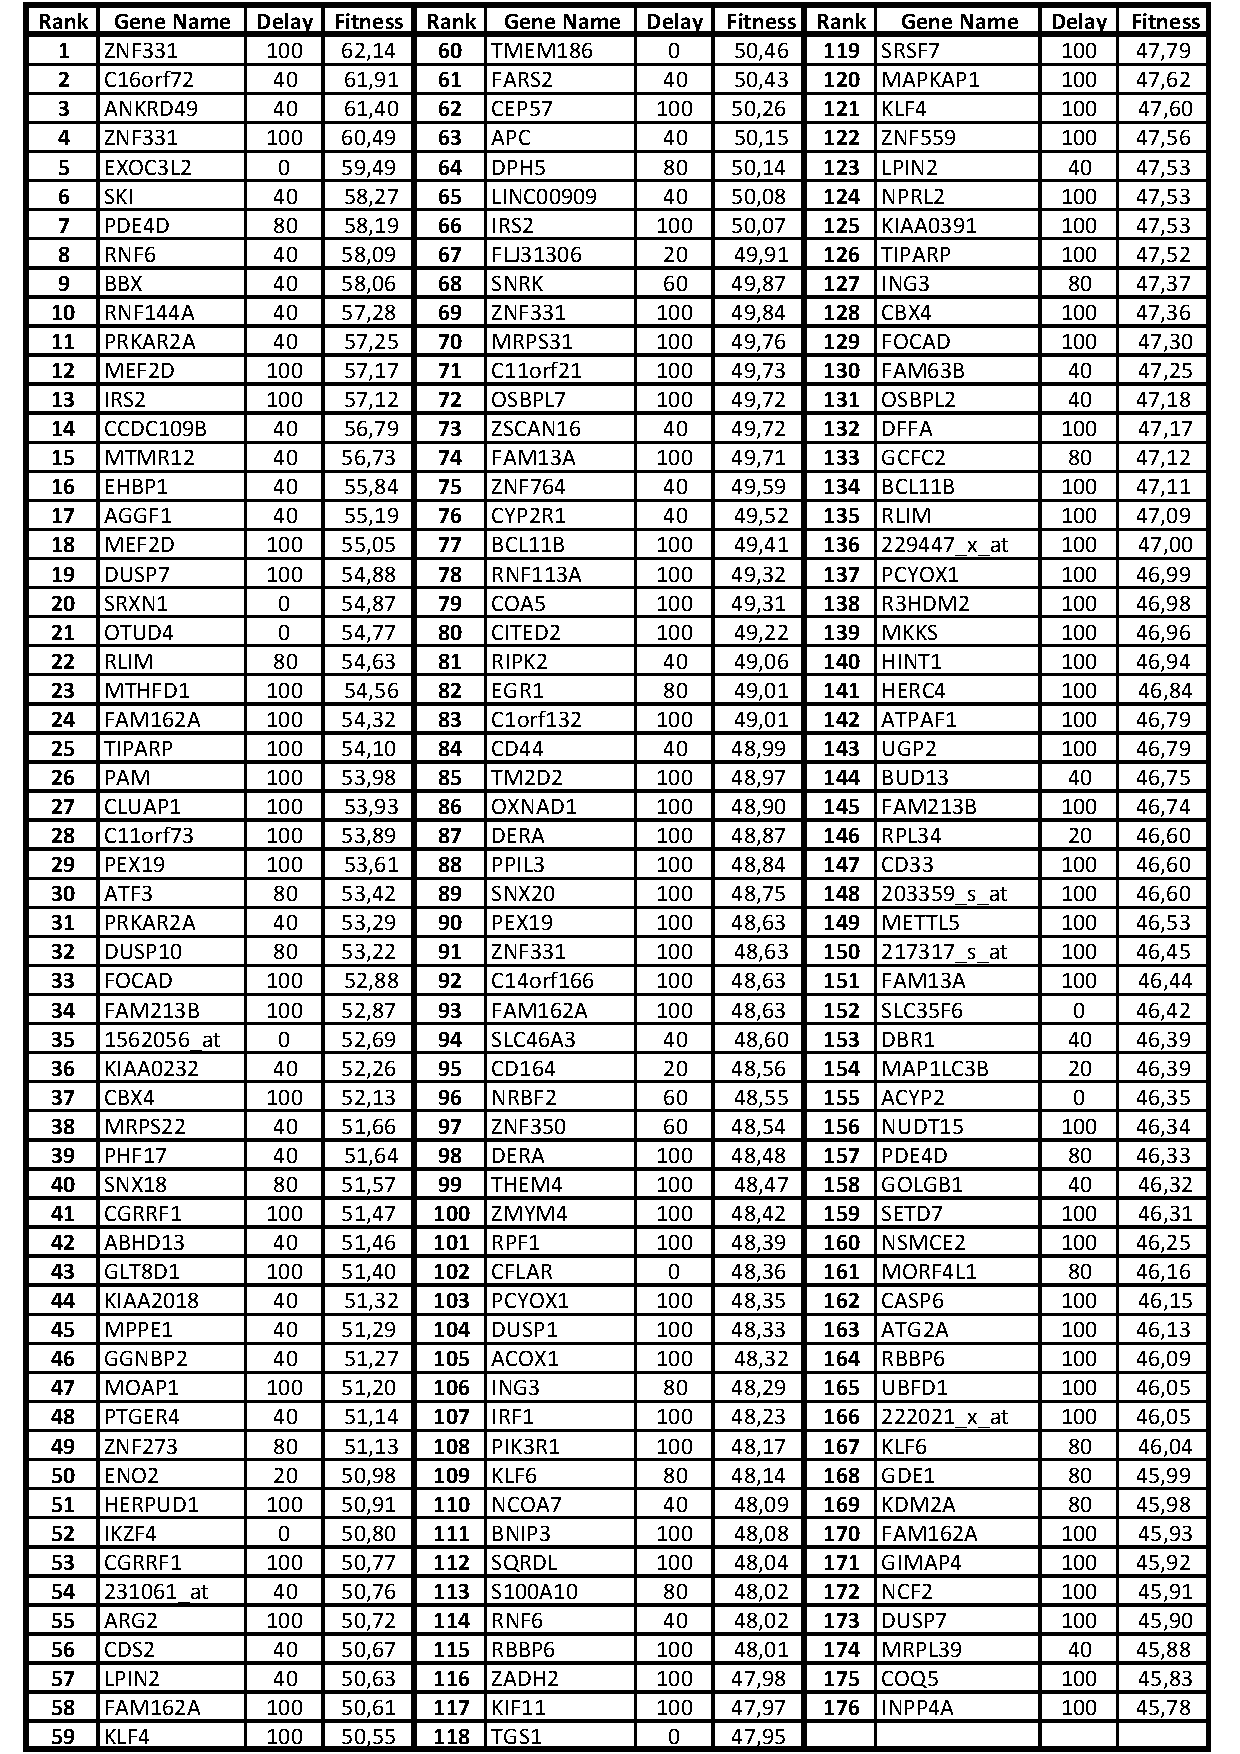
\includegraphics[scale=0.6]{Fig3SM.pdf}
  \caption{\textbf{Highest ranked 176 transcripts, corresponding to 161 genes, according to our approach.} First column: ranking, in descending order based on fitness scores. Second column: name of the gene, or Affymetrix probe-ID (a unique identifier) where multiple probe-IDs were associated to one name. Third column: delay (measured in minutes) corresponding to the model which received the highest fitness for that transcript as a regulator of FOXP3, for the second donor. Fourth column: actual value of the fitness score defined in Eq. \eqref{fitness}, for that model.
}
  \label{SupTabComputational}
\end{figure*}

\clearpage



%======================================
%\section{Experimental methods}  \label{SI:ExperimentalMethods}
%======================================

%\enlargethispage*{1.7\baselineskip}
\enlargethispage*{\baselineskip}

%\sub
\section{EXPERIMENTAL SUBJECTS, \mbox{MODEL, METHODS DETAILS}}

\subsection{Regulatory T Cell Sorting and Culture}
Informed consent was obtained from the healthy blood donors through the Red Cross Luxembourg and study procedures have been approved by the ethic committee of the Red Cross Luxembourg. Buffy coats from healthy male donors of unknown age were provided by the Red Cross Luxembourg and. Isolation of human Tregs were performed using similar methods as we described elsewhere \citep{Danileviciute2019.12.20.884809}. The RosetteSepac Human CD4$^{+}$ T cell Enrichment Cocktail (15062, Stemcell) was added to undiluted blood at a concentration of 50 $\mu$l/ml and incubated for 30 min at 4 $^\circ$C. The blood was then diluted 2 times with FACS buffer (PBS + 2$\%$ FBS) and the CD4$^{+}$ cells were isolated by gradient centrifugation at 1200 g for 20 min, using Lympoprep (07801, StemCell) and SepMateac-50 tubes (85450, Stemcell). Primary natural regulatory T cells (CD4$^{+}$CD25$^{high}$CD127$^{low}$) were then sorted on a BD Aria III Flow cytometry cell sorter (BD Biosciences). CD4$^{+}$ T cells were stained for 30 min at with mouse monoclonal [RPA-T4] anti-human CD4 FITC (555346, BD Biosciences) (dilution 1:20), mouse monoclonal [M-A251] anti-human CD25 APC (555434, BD Biosciences) (dilution 1:20), mouse monoclonal [HIL-7R-M21] anti-human CD127 V450 (560823, BD Biosciences) (dilution 1:20) 4 $^\circ$C followed by 2 washing steps with FACS buffer (250 g, 10 min).

Sorted Treg were cultured in IMDM (21980-032, ThermoFisher Scientific) complete medium, supplemented with 10$\%$ heat-inactivated (56 $^\circ$C, 45 min) fetal bovine serum (FBS) (10500-064, ThermoFisher Scientific), 1x Penicillin+Streptomycin (15070-063, ThermoFisher Scientific), 1x MEM non-essential amino acids (M7145, Sigma-Aldrich) and 1x $\beta$-mercaptoethanol (21985-023, ThermoFisher Scientific) at 37 $^\circ$C, 7.5$\%$ CO$_2$. The medium was further supplemented with 100 U/ml of recombinant human IL2 (2238131, Novartis) for the culture of Tregs. For a maximum duration of 6 weeks, the Treg were restimulated every 7 days with irradiated Epstein Barr virus (EBV) (strain B95-8, VR-1491, ATCC) transformed B cells (EBV-B cells), at a 1:1 ratio to expand and maintain the culture. A RS2000 X-Ray Biological Irradiator was used to irradiate the EBV-B cells (Rad Source Technologies) for 30 minutes with a total of 90 Gy. 
On a regular basis, the Tregs were characterized by Flow Cytometry for their expression of CD4, CD25, FOXP3 and Helios and discarded if the expression of FOXP3 and/or Helios was apparently decreased.


%\sub
%\section{EXPERIMENTAL METHOD DETAILS}
\enlargethispage*{\baselineskip}

%\sub
\subsection{Flow Cytometry for Treg Characterisation}
Extracellular markers were stained in FACS buffer for 30 min at 4 $^\circ$C, followed by 3 washing steps (250 g, 10 min). Fixation, permeabilization and staining of intracellular markers was performed using the True-Nuclear Transcription Factor Buffer Set (424401, BioLegend) and following the manufuacturers instructions. The antibodies used for the characterisation are in the  the following: mouse monoclonal [RPA-T4] anti-human CD4 BUV395 (564724, BD Biosciences) (dilution 1:100 ), mouse monoclonal [M-A251] anti-human CD25 FITC (555431, BD Biosciences) (dilution 1:100), mouse monoclonal [22F6] anti-human Helios Pacific blue (137220, BioLegend) (dilution 1:100), mouse monoclonal [206D] anti-human FOXP3 Alexa Fluor 647 (320114, BioLegend) (dilution 1:20). LIVE/DEAD® Fixable Near-IR Dead Cell Stain (L10119, ThermoFisher Scientific) (dilution 1:500).

%\sub
\subsection{Treg siRNA Knockdown and Stimulation} 
The P3 Primary Cell 4D-Nucleofector X Kit L (V4XP-3024, Lonza) was used for the knockdown of the targeted genes, using 90 $\mu$l P3 Primary cell solution and 100 pmol of corresponding si$_{RNA}$ (resuspended in 10 $\mu$l RNAse-free H2O): si$_{Non-Specific}$ (si$_{NS}$ or si$_{CTL}$) (sc-37007, Santa Cruz), si$_{NRBF2}$ (SI00139118, Qiagen), si$_{NCOA7}$ (SI02649668, Qiagen), si$_{MAP1LC3B}$ (SI04200735, Qiagen), si$_{PDE4D}$ (SI05587666, Qiagen), si$_{RNF14}$ (SI00113582, Qiagen). The Amaxa 4D-Nucleofector X System (Lonza) was used to perform the electroporation and siRNA transfection according to the manufacturers recommended program for primary human T cells. After transfection, the Tregs were transferred into a 12-well plate with pre-warmed complete medium, supplemented with 100 U/ml IL-2, and kept at 37 $^\circ$C for 24 h before being stimulated with 25 $\mu$l/ml of solutble antibodies (Immunocult Human CD3/CD28 T Cell Activator) (10971, Stemcell) \mbox{in a 24-well plate for 5, 10 and 15 h.}

%\sub
\subsection{RNA Extraction}
RNA was extracted using the RNeasy Mini Kit (74106, Qiagen), following the manufacturers instructions and including the digestion of genomic DNA with DNAse I (79254, Qiagen). The cells were lysed in RLT buffer (Qiagen), supplemented with 1$\%$ beta-Mercaptoethanol (63689, Sigma-Aldrich). The NanoDrop 2000c Spectrophotometer (Thermo Fisher Scientific) was used to measure the RNA concentration and its quality was checked by assessing the RNA integrity number (RIN) using the Agilent RNA 6000 Nano kit (5067-1511, Agilent) and the Agilent 2100 Bioanalyzer Automated Analysis System (Agilent), according to the manufacturers protocol. Only the samples with RIN of 8 or higher were considered for further analysis.

%\sub
\subsection{cDNA Synthesis}
A maximum of 500 ng of RNA was used for human cDNA synthesis, using the Superscipt IV First Strand Synthesis System (18091050, ThermoFisher Scientific) and following the manufacturers instructions. For the first step the mastermix contained following components (per sample): 0.5 $\mu$l of 50 $\mu$M Oligo(dT)20 primers (18418020, ThermoFisher Scientific), 0.5 $\mu$l of 0.09 U$\mu$l Random Primers (48190011, ThermoFisher Scientific), 1 $\mu$l of 10 mM dNTP mix (18427013, ThermoFisher Scientific) and RNAse free water for a final volume of 13 $\mu$l in 0.2 ml PCR Tube Strips (732-0098, Eppendorf). The reaction tubes were transferred into a C1000 Touch Thermal Cycler (Bio-Rad) or UNO96 HPL Thermal Cycler (VVR) and subjected to the following program: 5 min at 65 $^\circ$C, followed by 2 min at 4 $^\circ$C. For the second step, the  reaction mix was supplemented with 40 U RNaseOUT Recombinant Ribonuclease Inhibitor (10777019, ThermoFisher Scientific), 200 U SuperScript IV Reverse Transcriptase (18090050, ThermoFisher Scientific),  a final concentration of 5 mM Dithiothreitol (DTT) (70726, ThermoFisher Scientific) and 1x SSIV in a total reaction volume of 20 $\mu$l. The thermocycler program for the second step was the following: 50 $^\circ$C for 10 min, then 80 $^\circ$C for 10min and 4 $^\circ$C until further usage. The obtained cDNA was then 5x diluted with nuclease-free water to a final volume of 100 $\mu$l.

%\sub
\subsection{Quantitative Real-Time PCR (qPCR)} 
The reaction mix per sample for quantitative real-rime PCR (qPCR) contained: 5$\mu$l of the LightCycler 480 SYBR Green I Master Mix (04707516001, Roche), 2.5 $\mu$l cDNA and 2.5 $\mu$l primers in a total reaction volume of 10 ul. The reaction was performed in a LightCycler 480 (384) RT-PCR platform (LightCycler 480 (384), Roche), using the LightCycler 480 Multiwell 384-well plates (04729749 001, Roche) and LC 480 Sealing Foil (04729757001, Roche). The temperature program for qPCR was the following: 95 $^\circ$C for 5 min; 45 cycles of (55 $^\circ$C for 10 s, 72 $^\circ$C for 20 s, 95 $^\circ$C for 10 sec); meltingcurve (65-97 $^\circ$C). The results were analysed with the LightCycler 480 SW 1.5 software. Primers used for qPCR: RPS9 (QT00233989, Qiagen) as a reference gene, NRBF2 (QT00061936, Qiagen), NCOA7 (QT00033922, Qiagen),  FOXP3 (QT00048286, Qiagen) and MAP1LC3B (QT00055069, Qiagen).

%\sub
\subsection{Western Blotting}
Proteins were separated in Novex WedgeWell 4-20$\%$ Tris-Glycine Gels (XPO4202Box, Invitrogen), using the Novex Tris-Glycine SDS Running buffer (LC2675-4, Invitrogen). The proteins were transferred (dry transfer) using an iBlot2 Gel Transfer Device (IB21001, Invitrogen) and iBlot2 PVDF stacks (IB24002, Invitrogen). After the transfer the membranes were blocked in 5$\%$ milk in PBS with 0.2$\%$ Tween20 (PBS-T) for 1 hour at room temperature with gentle shaking before being incubated overnight at 4 $^\circ$C with the primary antibodies: rabbit monoclonal [15H7L3] anti-human NRFB2 (702920, ThermoFisher Scientific) (dilution 1:5000), rabbit polyclonal [FL-335] GAPDH (sc-25778, Santa Cruz Biotechnology) (dilution 1:200), mouse monoclonal [206D] FOXP3 (320102, Biolegend) (dilution 1:100), diluted in 5$\%$ BSA in PBS-T with 0.025$\%$ sodium azide. The next day the membrane was washed three times for 10 min before and after incubation with secondary goat anti-rabbit HRP-coupled antibodies (172-1019, Bio-Rad). The proteins were detected using the Amersham ECL Prime Western Blotting Detection Reagent (RPN2232, GE Healthcare Life Sciences) and visualized on the ECL Chemocam Imager (INTAS). If needed, the contrast and brightness of the obtained whole picture was adjusted using the Fiji ImageJ software.

%\clearpage

\begin{figure*}[ht!]
\centering
  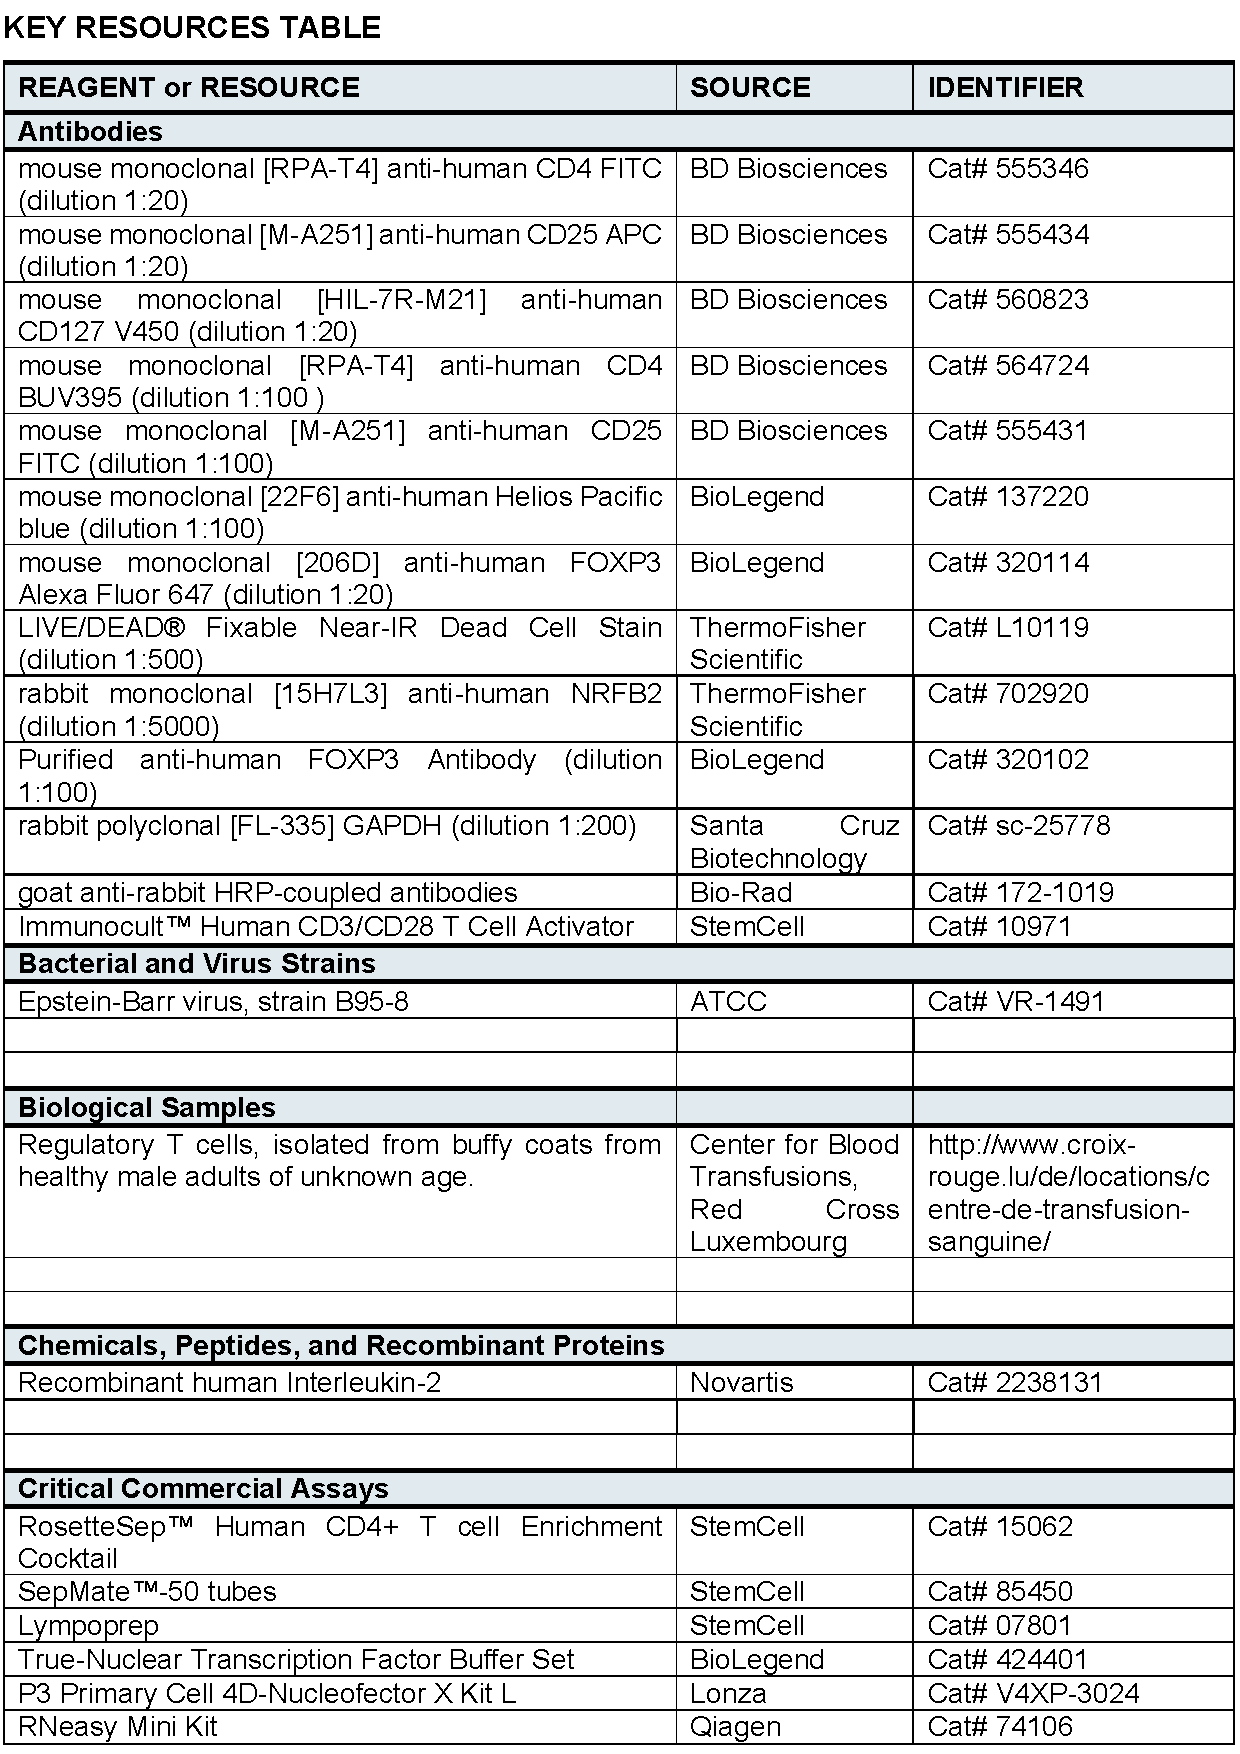
\includegraphics[scale=0.63]{Fig4aSM.pdf} % 0.63
\end{figure*}

%\clearpage

\renewcommand{\figurename}{Table}
\renewcommand{\thefigure}{S2}
\begin{figure*}[ht!]
\centering
  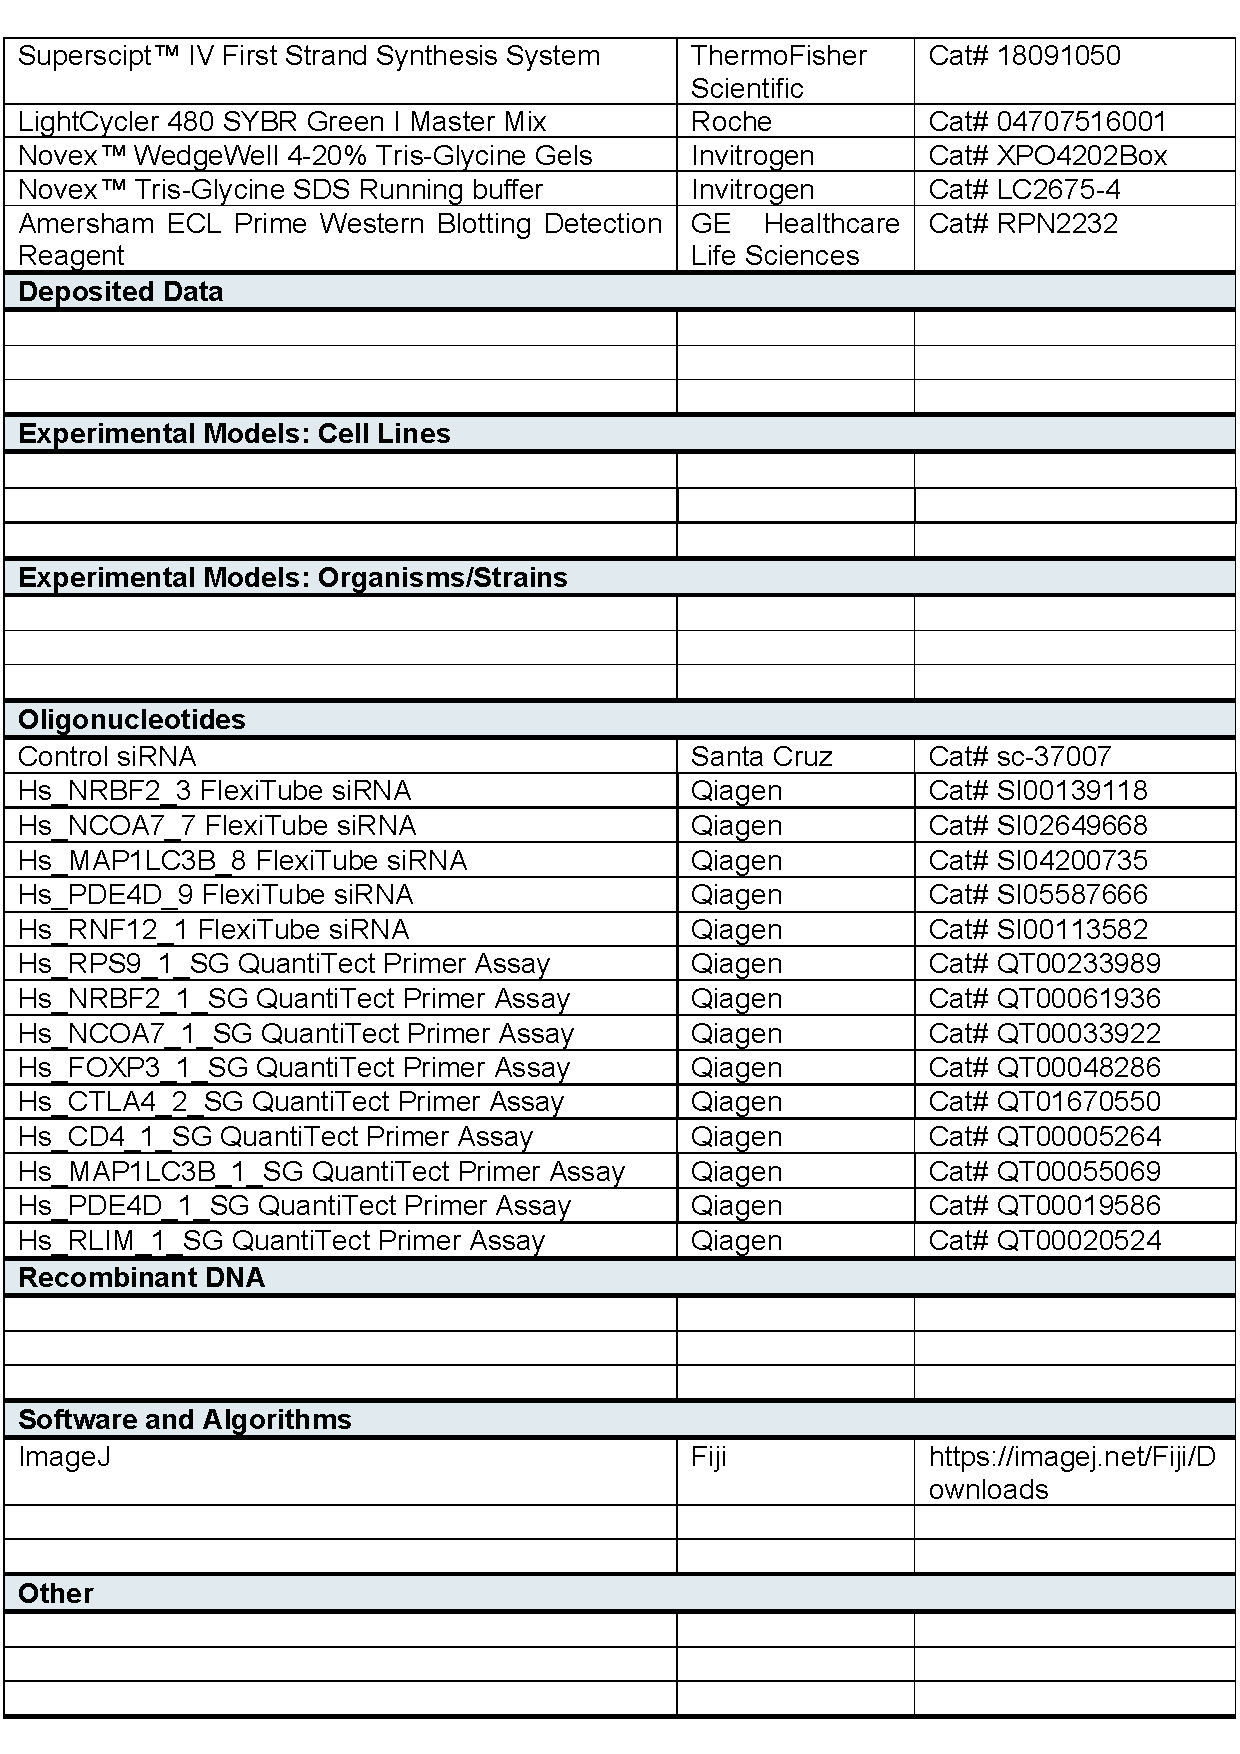
\includegraphics[scale=0.63]{Fig4bSM.pdf} % 0.63
  \caption{\textbf{Key Resources.} Materials employed for the experimental methods described in the text.
  \label{SupTabExperimental}
}
\end{figure*}

%\clearpage
%\includepdf[pages=1-2]{Tables_Experimental.pdf}
%\thispagestyle{empty}
%\nopagebreak





\end{document}
%%================= END OF DOCUMENT =================